\section{Укладка графа. Планарные и плоские графы. Теорема Эйлера о связи числа вершин, ребер и 
граней в плоском графе.}

\begin{definition}
    Граф называется \textit{укладываемым на поверхности} $S$, если его
    можно изобразить на $S$ так, что никакие два ребра не пересекутся во
    внутренних точках, само такое изображение графа называется \textit{укладкой графа
    на поверхности} $S$.
\end{definition}

\begin{definition}
    Если граф является укладываемым на плоскости, то он
    называется \textit{планарным}.
\end{definition}

\begin{definition}
    Любая укладка планарного графа на плоскости называется его
    \textit{плоской укладкой (плоским графом)}.
\end{definition}

Пример. Граф на рисунке а) является планарным, но не плоским. На рисунке
б) граф из пункта а) изображен по другому, без пересечений во внутренних
точках ребер, он является планарным и плоским.
\begin{figure}[h]
    \centering
    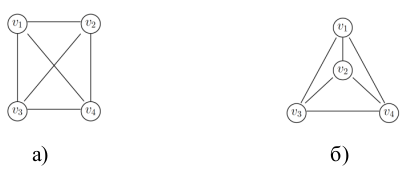
\includegraphics[scale=0.5]{30.png}
\end{figure}

Задача. Любое дерево является планарным графом.

\begin{definition}
    Пусть дана плоская укладка графа $G$. \textit{Гранью графа} $G$
    называется множество точек плоскости, каждую пару которых можно
    соединить кривой, не проходящей через вершины и ребра графа.
\end{definition}

\begin{definition}
    Грань, являющееся неограниченной областью плоскости,
    называется \textit{внешней гранью}, остальные грани называются \textit{внутренними}.
\end{definition}

Любая грань ограничена некоторым замкнутым маршрутом (не обязательно
циклом, в таком маршруте могут повторяться вершины и ребра).

Пример. На рисунке ниже отмечены грани плоского графа: 1,2,3 -- внутренние,
4 -- внешняя.

Внешняя грань ограничена замкнутым маршрутом $v_1 v_2 v_3 v_8 v_9 v_8 v_7 v_1$
\begin{figure}[h]
    \centering
    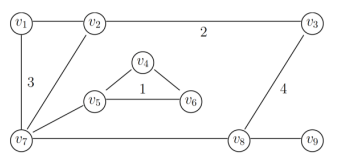
\includegraphics[scale=0.5]{30_2.png}
\end{figure}

\begin{theorem}
    (Эйлера) Если связный плоский граф имеет $n$ вершин, $r$ ребер и $q$
    граней (включая внешнюю), то справедливо равенство
    \begin{align*}
        n-r+q=2
    \end{align*}
\end{theorem}

\begin{proof}
    Рассмотрим $G(V, E)$ -- граф, у которого $n$ вершин, $r$ рёбер, $q$
    граней.

    Найдем его остовное дерево. В нем будет $n$ вершин, $n - 1$ рёбер, 1 грань
    (внешняя). Для полученного остовного дерева равенство выполняется:
    \begin{align*}
        n-r+q=n-(n-1)+1=2
    \end{align*}
    Будем добавлять в остовное дерево по одному ребру. Так как граф плоский,
    то при этом каждый раз будет добавляться один замкнутый маршрут, а
    значит, одна грань будет отделяться, то есть на одну грань каждый раз будет
    становиться больше. Так как число граней и ребер стоят в равенстве с
    разными знаками, то сумма меняться не будет. Так можно дополнить
    остовное дерево до самого графа, при этом равенство $n - r + q = 2$
    сохранится.
\end{proof}